\documentclass[11pt]{article}
  
%%%%Packages:

%Page Setup
\usepackage{xcolor}
\usepackage[a4paper, total={6in, 9.5in}]{geometry}
\pagecolor{white}

\setlength\parindent{0pt} %Paragraph indentation


%%%Packages
%Mathematics:
\usepackage{amsmath}
\usepackage{amssymb}
\usepackage{cancel}

%Programming
\usepackage{listings}

%QCircuits
\usepackage[braket,qm]{qcircuit}

%Ornaments:
%Frames around equations:
\usepackage{empheq}
\setlength\fboxsep{0.2cm}
%Ghost space for exponents
\newcommand\medstrut{\rule{0pt}{14pt}}
\newcommand\bigstrut{\rule{0pt}{18pt}}

%Calligraphic Characters:
\usepackage{ mathrsfs }
\usepackage[percent]{overpic}

%Graphics
\usepackage{tikz}
\usepackage{xcolor}
\usepackage{pgfplots}
\pgfplotsset{compat=1.5}
\usepgfplotslibrary{groupplots}
\usepgfplotslibrary{fillbetween}
\usetikzlibrary{patterns}

\usepackage{subcaption} %Subfigures



\begin{document}


\begin{center}
{\Huge \textbf{Task 2}}\\
\medskip
\today
\medskip
\hrule
\hrule
\end{center}

\medskip

\section{The Problem}

Implement a circuit which returns $|00 \rangle$ and $|11\rangle$ with equal probability. \\
\\
%
\emph{Requirements}: \\
%
- Circuit should consist only of \textsf{CNOT}s, \textsf{RX}s and \textsf{RY}s. 
Start from all parameters in parametric gates being equal to 0. 
You should find the right set of parameters using gradient descent (you might use more advanced optimization methods if you like). \\
%
- Simulations must be done with sampling - i.e. limited number of measurements per iteration and noise. \\
%
- Compare the results for different numbers of measurements: 1, 10, 100, 1000. \\
\\
%
\emph{Bonus question}:\\
%
How to make sure you produce state $|00\rangle +|11\rangle$ and not $|00\rangle -|11\rangle$ ?

\section{Solution}

Here I present a solution using two qubits. The basic idea is to use a parameterized $\textsf{RY}(\theta)$ gate and use a controlled-not gate to copy the phase-shifted state. 
%
$$
\Qcircuit @C=1em @R=1em {
\lstick{\ket{0}} & \gate{\textsf{RY}(\theta)} \qw & \ctrl{1} & \rstick{} \qw \\ 
\lstick{\ket{0}} & \qw & \targ & \rstick{} \qw
}
$$
\\
The parameterized gate is defined as:
%
\begin{align}
\textsf{RY}(\theta) = \textsf{exp} \left(-\frac{i\theta}{2}\textsf{Y}\right) = \textsf{cos}(\theta/2) \ \mathbb{I} - i\textsf{sin}(\theta/2) \textsf{Y}
\end{align}

so that when we apply it to one of the initial qubits, we get:
%
\begin{align}
\textsf{RY}(\theta) \ket{0} =  \textsf{cos}(\theta/2) \ket{0} + \textsf{sin}(\theta/2) \ket{1}
\end{align}

and thus the total state so far is:
%
\begin{align}
\ket{\psi(\theta)} = \textsf{cos}(\theta/2) \ket{00} + \textsf{sin}(\theta/2) \ket{10}
\end{align}

Next, the \textsf{CNOT} gate will flip the second qubit only in the second term (because of linearity). Our output state will be:
%
\begin{align}
\ket{\psi_{\text{out}}(\theta)}=\textsf{CNOT}\ket{\psi(\theta)} = \textsf{cos}(\theta/2) \ket{00} + \textsf{sin}(\theta/2) \ket{11}
\end{align}

We have now control over the output state by varying the parameter $\theta$: when $\theta=0$ we can produce the $\ket{00}$ state only and if $\theta = \pi/2$, we get:
%
\begin{align}
\ket{\psi_{\text{out}}(\pi/2)}= \frac{1}{\sqrt{2}} \big( \ket{00} +  \ket{11} \big)
\end{align}

which is a state with equal probabilities for $\ket{00}$ and $\ket{11}$:
%
\begin{align}
|\langle 00 | \psi_{\text{out}} \rangle |^2 = |\langle 11 | \psi_{\text{out}} \rangle |^2 = 0.5
\end{align}

 Notice that if we set $\theta = -\pi/2$, we will obtain the antisymmetric state $\ket{\psi_{\text{out}}(-\pi/2)}= \frac{1}{2} \big( \ket{00} -  \ket{11} \big)$, which still gives equal probabilities.

\section{Implementation}

When implementing this solution on software, let's forget for a moment we know the desired values of the parameter and let's look for it using gradient descent. I have used the open source library \textsf{Cirq}, and its basic \emph{Controlled-not} and \emph{Rotate-Y} gates. Also, I have introduced noise channels that apply some Pauli gate with a probability $p$ and the identity with probability $1-p$. The code is in a \textsf{Jupyter Notebook} done with coLab, because I think it's easier to read it in blocks and it should be quick to access online.
\\

The gradient descent method allows us to vary the parameter in such a way that a desired function has zero derivative. Here I used a function that adds the different amplitudes as measured by the sampling:
%
\begin{align}
\epsilon(\textsf{counts}) = \textsf{counts}(\ket{01}) + \textsf{counts}(\ket{10}) +(\textsf{counts}(\ket{00})-\textsf{counts}(\ket{11})\,)^2
\end{align}

where I divided $\textsf{counts}(\ket{\cdot}) = \textsf{frequencies}(\ket{\cdot})/N_{\text{samples}}$ to make the errors commensurate with the probabilities, and where there's an additional term to try to reduce the difference between the desired states.
\\

The strategy now is to update the parameter $\theta$ (which we can initialize randomly between $(-\pi, \pi)$ with the variation in the function $\epsilon$:
%%
\begin{align}
\Delta \epsilon &= \epsilon(\textsf{new  counts}) - \epsilon(\textsf{prev. counts})\\
\theta_\text{new} &= \theta_\text{old} - \gamma \Delta \epsilon -\textsf{sign}(\Delta \epsilon)\epsilon 
\end{align}

where the last term allows us to avoid a local maximum by penalizing (according to the sign of the variation) a high error. We choose a small step $\gamma$ which here we set by hand (e.g. 0.01), and iterate the procedure until $\Delta \epsilon$ is below a desired threshold.

\subsection{Bonus}

If we wish to ensure we obtain the symmetric state $\ket{\psi_{\text{out}}}= \frac{1}{\sqrt{2}} \big( \ket{00} +  \ket{11} \big)$, we have to make sure that we don't fall into the negative minimum $\theta = -\pi/2$. We enforce this by adding another penalizing term a negative parameter (which we denote here with a Heaviside $\Theta$ function, or unit step):

\begin{align}
\theta_\text{new} &= \theta_\text{old} - \gamma \Delta \epsilon -\textsf{sign}(\Delta \epsilon)\epsilon + \Theta(-\theta) 
\end{align}

\section{Results}

Here I have chosen a small noise $p = 0.05$ which also gives an order of magnitude for the error threshold: the iterations stop when $\epsilon < 0.05$, or when they are more than $100$. The number of samples has to be high enough to ensure that we get a meaningful error function: If we just take 1 sample, the frequency count   is just 1 so the error is always 1 ($\Delta \epsilon = 0$ and no gradient descent). We expect that the averages of these counted quantitites converge towards the expected value and so we begin to see more coherent results as we increase the number of samples.\\

Below are some examples of the observed behavior, for $N_{\text{samples}} \in \{10,100,1000\}$: 


\begin{figure}[h!]
\centering
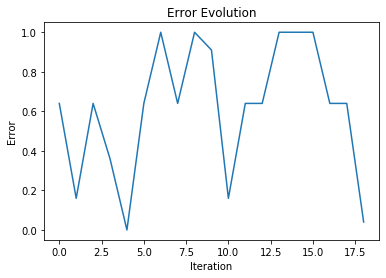
\includegraphics[scale=0.5]{error10}
\caption{Evolution of the error function with the number of iterations. Here the threshold for success in the variation of the parameter is $0.05$, but we also forced the code to run for at least 10 iterations before stopping. It eventually reached threshold again at 18 iterations.}
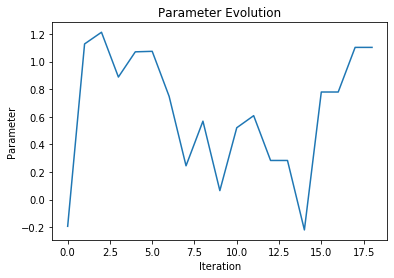
\includegraphics[scale=0.5]{parameter10}
\caption{Evolution of the varying parameter $\theta$. Since we are selecting the symmetric state, the evolution converges towards the expected value $\theta = \pi/2$, although the few number of samples can make the error very small without really reaching the best parameters.}
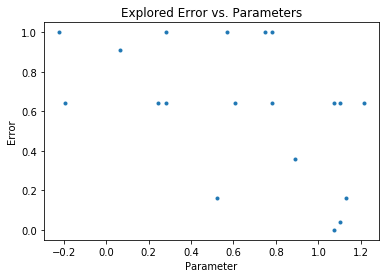
\includegraphics[scale=0.5]{explored10}
\caption{Relationship between the explored parameters and their calculated error, There is no clear relationship that can be inferred, again because of the small number of samples.}
\vspace{10pt}
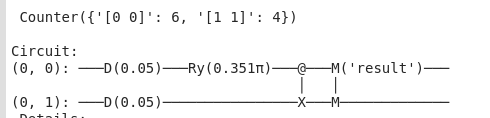
\includegraphics[scale=0.5]{result10}
\caption{Displayed frequency count and resulting circuit after the iterations. The parameter was close enough so that the counts are more or less similar. The final value for the $\textsf{RY}$ gate was $0.351 \pi$.}
\end{figure}



\begin{figure}[h!]
\centering
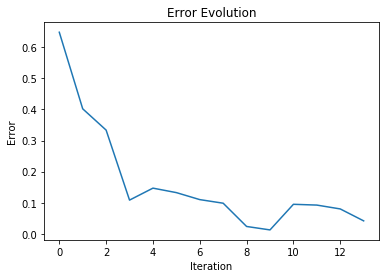
\includegraphics[scale=0.5]{error100}
\caption{Evolution of the error function with the number of iterations. The threshold for success in the variation of the parameter is $0.05$ and the higher number of samples (100) made this a smoother run towards some minimum.}
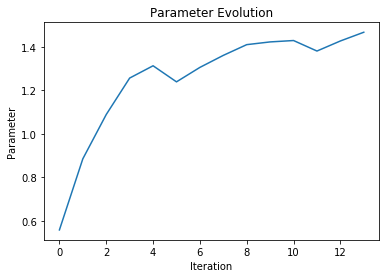
\includegraphics[scale=0.5]{parameter100}
\caption{Evolution of the varying parameter $\theta$. Since we are selecting the symmetric state, the evolution converges towards the expected value $\theta = \pi/2$}
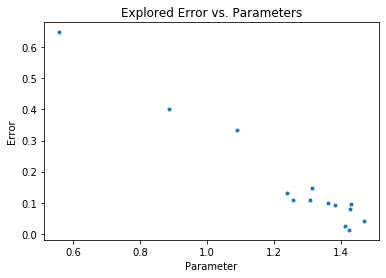
\includegraphics[scale=0.5]{explored100}
\caption{Relationship between the explored parameters and their calculated error, showing both the minimum of convergence and also the maximum error at $\theta = \pi$ that we want to avoid.}
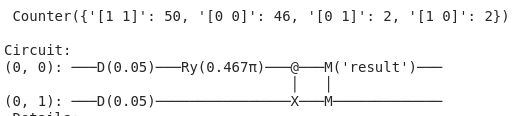
\includegraphics[scale=0.5]{result100}
\caption{Final frequency count and resulting circuit. Notice the counter of states $|01\rangle$ and $|10\rangle$ is not zero because this time the noise in the model (shown by the ``$\textsf{D}$'' gates at 0.05 percent) added some extra hits in some samples . The final value for the $\textsf{RY}$ gate was $0.467 \pi$, which is what we expect for the symmetric state.}
\end{figure}

\begin{figure}[h!]
\centering
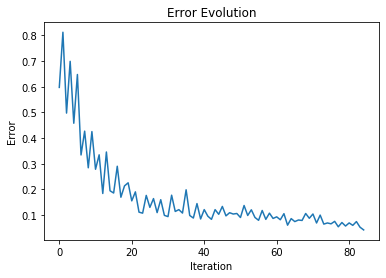
\includegraphics[scale=0.5]{error}
\caption{Evolution of the error function with the number of iterations,now for 1000 samples on each run. The threshold for success in the variation of the parameter is $0.05$ and the convergence is quite clear, although the noise can cause some wiggling in the measured error.}
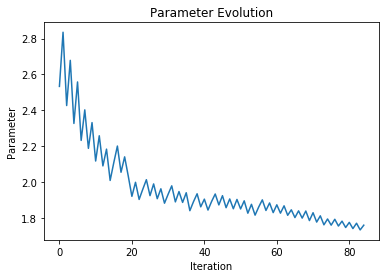
\includegraphics[scale=0.5]{parameter}
\caption{Evolution of the varying parameter $\theta$. Since we are selecting the symmetric state, the evolution converges towards the expected value $\theta = \pi/2$}
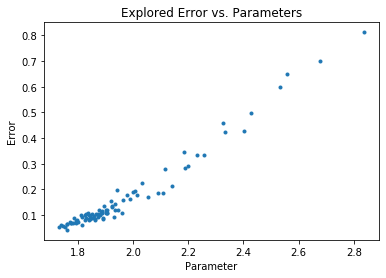
\includegraphics[scale=0.5]{explored}
\caption{Relationship between the explored parameters and their calculated error, showing both the minimum of convergence and also the maximum error at $\theta = \pi$ that should be avoided, in a different region, since we started at $\theta \sim 2.6$}
\vspace{10pt}
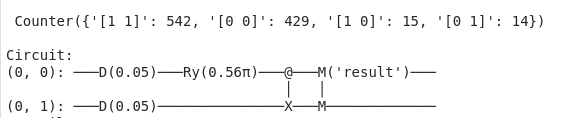
\includegraphics[scale=0.5]{result}
\caption{Displayed frequency count and resulting circuit after the iterations. Notice the counter of states $|01\rangle$ and $|10\rangle$ is not zero because we have added noise to the model, shown by the ``$\textsf{D}$'' gates at 0.05 percent. The final value for the $\textsf{RY}$ gate was $0.56 \pi$, which is what we expect for the symmetric state, and the noise we put into the circuit.}
\end{figure}

\end{document}